\en

\section{Tool functionalities}
\label{subsec:func}

We proposes three main functionalities for the user in the tool, which are named duplication explorer, function information
and duplication relatory. Each of the functionalities recevies their adequated parameters to execute, with a exception
of a optional parameter shared by all of them, which is minimum similarity per query. The minimum similarity per query is different
from the siminum similarity presented in \ref{subsec:setup}, as it enables a volatile change in the minimum similarity
interested in a query specific context. There is a explanation of each of the main functionalities throughout this section.

\subsection{Duplication explorer}

The duplication explorer is the principal functionality of our tool, the functionality purpose is to expose for the user the code duplication
pairs found by our tool. We implement optional filters methods to enable more complex queries, which are described below. A example
of the functionality usage can be found in the figure \ref{fig:explorer_ex}.


\begin{itemize}
	\begin{item}
		\textbf{Sorting filter:} This filter enables the user to sort the resuls by similarity of the functions pairs or 
		by the number of duplicated lines. By default the tool sorts by similarity and the user can pass a sort parameter to change
		the sorting method.
	\end{item}

	\begin{item}
		\textbf{Limiter filter:} This filter receives a number parameter named limiter by the user, which limits the number of results
		showed to the user by this given number.
	\end{item}

	\begin{item}
		\textbf{Pattern filter:} This filter make the explorer ignore every pair of duplicated functions that does not match a pattern
		given by the user as a parameter. We say that a function matches a pattern if the string formed by the concatenation of
		the relative path of the code file plus the function name. The user can define if both functions or at least one of the 
		functions in the pair need to match the pattern by given a specific parameter.
	\end{item}
\end{itemize}

\begin{figure}
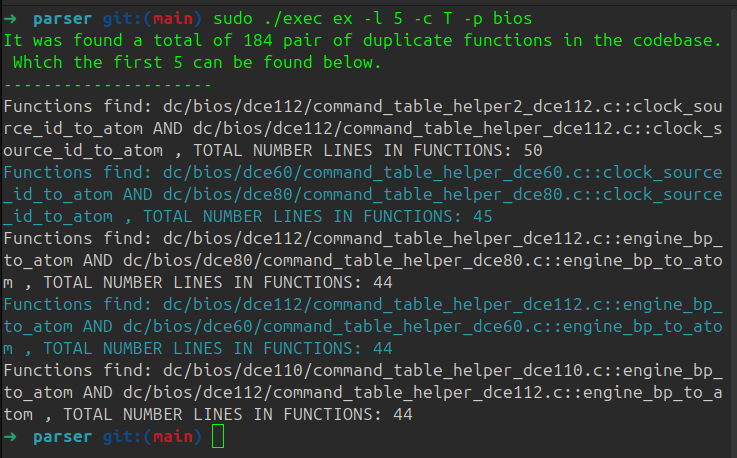
\includegraphics[scale=0.5]{explorer_example}
\caption{Explorer Example}
\label{fig:explorer_ex}
\end{figure}


\subsection{Function information}

The Function information purpose it to give a more in depth information about a specific function. The functionality inform the user
about the relative path, the function name and the lines the function exist in the code file that the function is contained for the
function that the user is interested and every function that is a duplication of it. As there ca nbe multiple functions with the 
same name in a codebase, we distinguish then by the user providing a pattern string and we use the first function find that match
the pattern. We say that a function matches a pattern if the string formed by the concatenation of the relative path of the 
code file plus the function name. 
A example of the functionality usage can be found in the figure \ref{fig:function_ex}.


\begin{figure}
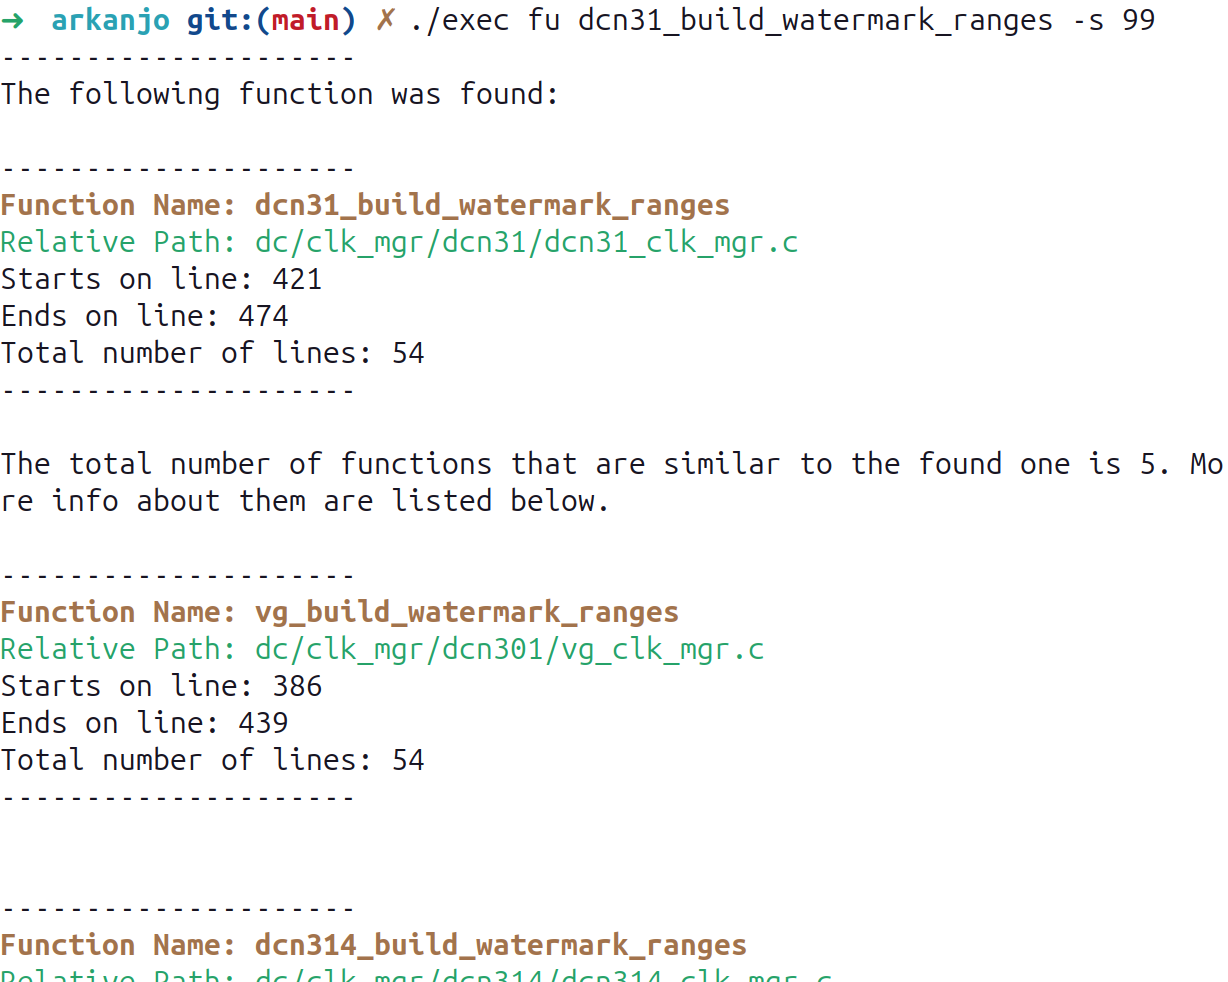
\includegraphics[scale=0.5]{function_example}
\caption{Function Example}
\label{fig:function_ex}
\end{figure}


\subsection{Duplication relatory}

The duplication relatory purpose is to give a overview of the input codebase. The functionality extract the information
of how much lines of duplicated code is found per folder in the codebase and present it to the user in a reasonable format. To extract
the information, we use the Code Duplication Database to list the code duplications, and the temporary code to know how much lines of
duplicated code contains in each of the functions. (DO I TALK ABOUT THE TRIE USAGE TO MAINTAIN THE HIERARCHICAL TREE STRUCTURE? I 
THINK NOT). A example of the functionality usage can be found in the figure \ref{fig:relatory_ex}.

\begin{figure}
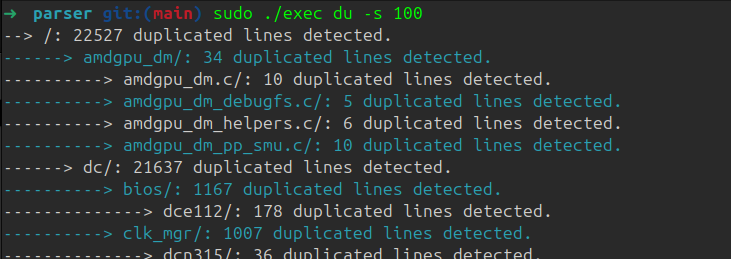
\includegraphics[scale=0.5]{relatory_example}
\caption{Function Example}
\label{fig:relatory_ex}
\end{figure}





